General equation of straight line is given by:\\
\begin{align}
    \vec{n}^T \vec{x} = c 
\end{align}   
\vspace{0.5 cm}
$\vec{n}$ will be same because both lines are parallel. \\
\begin{align}
    \vec{n} = \begin{pmatrix} 2  \\ 5 \end{pmatrix}
\end{align}
Passing through mid point $\vec{M}$ of $\vec{A}, \vec{B}$:
\begin{align}
  \vec{M} = \frac{ \vec{A} + \vec{B}}{2}
\end{align}
\begin{align}
    \vec{n}^T (\vec{x} - \vec{M}) = 0 \\
    \vec{n}^T \vec{x} = \vec{n}^T \vec{M} 
\end{align}

So, the mid point $\vec{M}$ is :
\begin{align}
   \vec{M} = \frac{\begin{pmatrix} -7  \\ 3 \end{pmatrix} + \begin{pmatrix} 5 \\ -11 \end{pmatrix}}{2}  = \begin{pmatrix} -1  \\ -4 \end{pmatrix}  \\
   \vec{n}^T \vec{x} =  \begin{pmatrix} 2 & 5 \end{pmatrix}\begin{pmatrix} -1  \\ -4 \end{pmatrix} = -22
\end{align}
So, the equation of line is :
\begin{align}
   \begin{pmatrix} 2 & 5 \end{pmatrix}\vec{x} = -22
\end{align}

\begin{figure}[t]
    \centering
    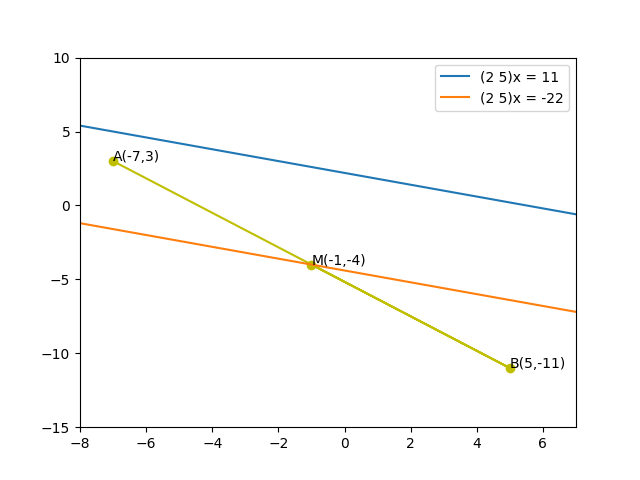
\includegraphics[width = \columnwidth]{./solutions/2/2/15/AI_assignment_2.png}
    \caption{Parallel Lines}
    \label{eq:solutions/2/2/15/fig:Lines}
\end{figure}

